\subsection{Systemarchitektur}
Abbildung \ref{img:Systemarchitektur}: \nameref{img:Systemarchitektur} zeigt die Systemarchitektur des zu entwickelnden Systems. Es handelt sich um eine Server-Client-Architektur, bei der die Instanzen über die REST-API-Schnittstelle kommunizieren.
\begin{figure}[H]
	\centering
	\setlength{\fboxsep}{1pt}
	\setlength{\fboxrule}{1pt}
	\fbox{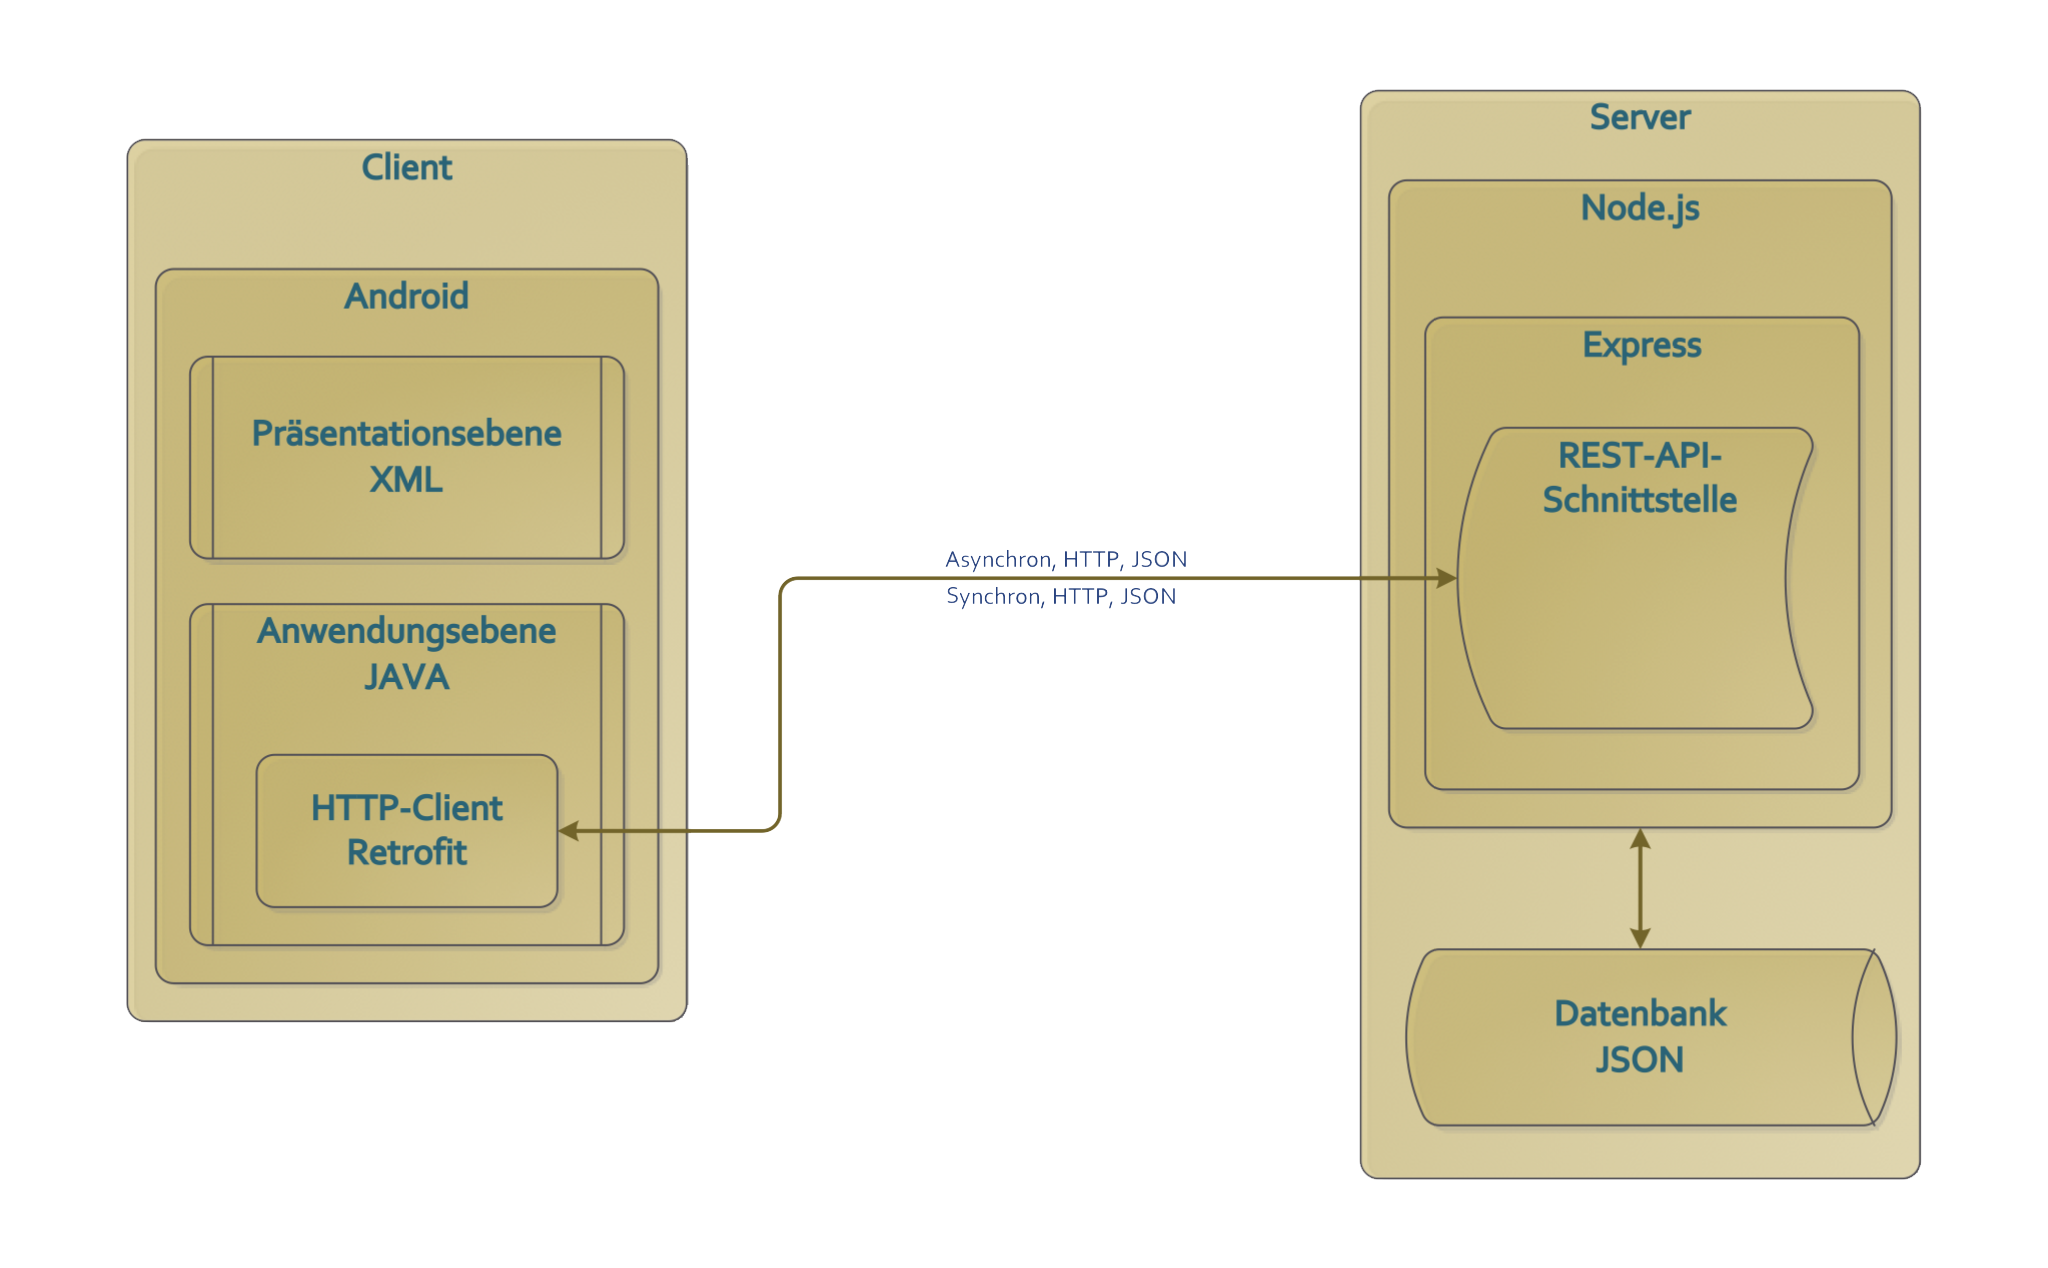
\includegraphics[width=1.0\textwidth]{images/systemarchitektur.png}}
	\captionsetup{justification=centering}
	\caption{Systemarchitektur}
	\label{img:Systemarchitektur}
\end{figure}
\subsubsection{Server-Client}
	In dem zukünftigen System für Android wird die Benutzeroberfläche von der Datenverwaltung getrennt. Dadurch kann das System in Zukunft plattformunabhängig sein. In weiteren Entwicklungsphasen könnte auch ein Client (Frontend) für das iOS-Betriebssystem implementiert werden, der ebenfalls mit dem Server (Backend) kommuniziert.\\
	Da eine direkte Kommunikation zwischen Systemkomponenten nicht erwünscht ist und kommunizierte Daten dauerhaft (persistent) und zentral gespeichert werden sollen, wurde eine Entscheidung gegen eine Peer-to-Peer-Architektur getroffen. Denn die Datenspeicherung für einzelne Komponenten wäre unsicher und würde ein Datenschutzrisiko darstellen.\\
	Die Client-Server-Architektur ist ebenfalls geeignet, da das System ein REST-spezifisches Design haben sollte. Zentrales Ressourcenmanagement ist eines der REST-Paradigmen, ermöglicht die Verwaltung vieler Benutzerdaten und gewährleistet einen bestimmten Sicherheitsstandard. Die Erweiterbarkeit, die diese Systemarchitektur ermöglicht, ist ein weiterer Grund, warum Client-Server als Architekturmodell ausgewählt wurde. 
\subsubsection{Server}
	Der Server ist das Zentrum des Systems und erledigt die Hauptarbeit. Kernaufgabe ist es, die vom Client empfangenen Daten in einer Datenbank zu speichern und danach mit Algorithmen zu prozessieren. Die Ergebnisse werden dem Client zur Verfügung gestellt. Der Server enthält eine REST-API-Schnittstelle über Framework Express.js, die für die Kommunikation mit dem Client verwendet wird. Die Entwicklung erfolgt in der Skriptsprache JavaScript in einer NodeJS-Umgebung.\\
	Aufgrund seiner unkomplizierten Struktur und Skalierbarkeit ist NodeJS ideal für das System. Darüber hinaus liegen bereits Erfahrungen in der Programmierung mit JavaScript und NodeJS aus der vorangegangenen Entwicklungsphase und der Implementierung eines Prototyps vor. Da das System REST-spezifisch sein sollte, ist die Verwendung von Framework Express.js geeignet.  
	\subsubsection{Client}
	Der Benutzer interagiert mit dem System über eine App auf seinem Android-Gerät und erhält eine Darstellung seiner verarbeiteten Daten. Bei der Implementierung der Benutzeroberfläche des Systems wurde eine Android-App anstelle einer Web-Anwendung ausgewählt. Dies scheint bei der Benutzer-System-Interaktion (user-system interaction) am sinnvollsten zu sein, da interaktive Arbeit am System ein einfacher und müheloser Vorgang ist, der in kurzer Zeit durchgeführt werden sollte, sodass eine Web-Applikation, die den Einsatz eines Browsers erfordert zu aufwendig wäre. Darüber hinaus müssen Webpages zunächst erstellt und für mobile Geräte optimiert werden und bei dem Umfang dieses Projektes wäre sogar ein Webserver erforderlich.\\
	Der Grund für die Wahl der Android-Plattform war auch die vorhandene Erfahrung mit Java. Retrofit eignet sich sehr gut als HTTP-Client für Android und Java. Er ist sehr flexibel im Design und ermöglicht das Senden und Empfangen von JSON- und XML-Dateien.\\
	Während die Anwendungsebene in Java programmiert wird, wird die Benutzeroberfläche des Clients durch XML dargestellt.
	\subsubsection{Datenbank}
	Die Datenbank ist mit dem Server verbunden und ermöglicht eine persistente Speicherung der Daten. Sie hostet Benutzerprofile und Benutzerereignisse und fungiert als Datenbanksystem für Lebensmittel- und Aktivitätsdaten.
	\subsubsection{Datenformat}
	Die Daten dieses Systems haben das JSON-Datenformat. JSON-Daten haben dieselbe Syntax wie JavaScript-Objekte, sodass die Verarbeitung der Daten in JavaScript einfach bleibt. JSON-Objekte können auch in Java gut verarbeitet werden, da passende Klassen implementiert werden können. Da der Server mit JavaScript und die Clients in Java programmiert sind, wurde entschieden, JSON zu verwenden. Zudem sind die verwendeten Daten nicht flexibel und immer fest strukturiert, weshalb auf die Verwendung von XML verzichtet wurde.
	\subsubsection{Protokolle}
	HTTP (HyperText Transfer Protocol) wird als Protokoll für die Datenübertragung verwendet, da der Server über eine REST-spezifische Architektur verfügt und JSON-Objekte über HTTP übertragen werden können.
	\subsubsection{Asynchrone und Synchrone Kommunikation}
	Die Kommunikation zwischen Server und Client kann sowohl synchron als auch asynchron erfolgen. Wenn der Benutzer Daten wie z. B. seine Blutzuckerwerte abrufen und anzeigen möchte, wird auf die nicht blockierende asynchrone Kommunikation zugegriffen, um sowohl bei erfolgreicher als auch bei fehlgeschlagener Anforderung ein Ergebnis zu erhalten. Beim Schreibvorgang, beispielsweise wenn der Benutzer ein neues Ereignis hinzufügt, erfolgt dies über eine synchrone Kommunikation.	
\subsection{Datenstrukturen}
	Die modellierten Datenstrukturen des Systems werden nachfolgend erläutert. Die dargestellten Datenstrukturen sind JSON-Objekte, für die auf dem Client entsprechende Klassen implementiert wurden.
	\subsubsection{Benutzerprofil}
	Ein Benutzerprofil enthält alle erforderlichen benutzerbezogenen Daten, die bei der Registrierung erstellt und später geändert werden können. Tagebucheinträge werden jedem zugeordneten Benutzer hinzugefügt. Für jeden dokumentierten Tag gibt es einen Eintrag mit einer ID, einem Datum und den Ereignissen. Ereignisse enthalten Informationen zu Uhrzeit, Blutzucker, Mahlzeit, BE/KE, Insulin-Einheiten und sportlicher Aktivität. Ein Datensatz für Mahlzeiten besteht aus einer Beschreibung und der Anzahl der Kalorien, Kohlenhydrate, Eiweiße und Fette. Sportliche Aktivitäten enthalten eine Beschreibung, die Dauer und die Anzahl der verbrannten Kalorien.
	\lstinputlisting{listings/benutzerprofil.json}
	\subsubsection{Beiträg und Kommentare}
	Ein Beitrag kann von einem Benutzer erstellt und von allen anderen Benutzern angezeigt werden. Um einem Benutzer einen Beitrag zuordnen zu können, erhält der Beitrag die Benutzer-ID und den Benutzernamen des Verfassers. Außerdem enthält jeder Beitrag seine zugehörigen Kommentare, die dieselbe Datenstruktur wie die Beiträge haben. Auf dem Client erbt die Comments-Klasse die Attribute der Post-Klasse. 
	\lstinputlisting{listings/beitrag.json}
	\subsubsection{Lebensmittel}
	Der Benutzer sollte in der Lage sein, seine Mahlzeiten zu dokumentieren. Dies erfordert eine Lebensmitteldatenbank, die verschiedene Lebensmittel enthält. Lebensmittel werden anhand ihrer ID, ihres Namens und ihrer Kategorie identifiziert und enthalten eine Menge und eine Einheit, anhand derer die Anzahl der Kalorien, Kohlenhydrate, Proteine und Fette bestimmt wird. Wenn der Benutzer die Menge der Mahlzeit angibt, werden die Nährstoffe basierend auf der Menge und der Einheit aus der Datenbank berechnet. 
	\lstinputlisting{listings/lebensmittel.json}
	\subsubsection{Sportart}
	Eine Sportartendatenbank soll es dem Benutzer auch ermöglichen, sportliche Aktivitäten zu dokumentieren. Um den Kalorienverbrauch einer Sportart zu berechnen, verwendet man das sogenannte metabolische Äquivalent (metabolic equivalent of task; MET). Ein MET entspricht einem Energieverbrauch von einer Kalorie pro kg Körpergewicht und Stunde. Eine Sportart besteht also aus ihrem Namen und der MET-Anzahl zur Berechnung des Kalorienverbrauchs.
	\lstinputlisting{listings/sportart.json}
\subsection{REST-Spezifikation}
	Die REST Spezifikation des Servers beschäftigt sich mit ihren Ressourcen und dessen HTTP-Methoden, die folglich erläutert werden.
	\subsubsection{Benutzer}
	\begin{itemize}
	\item Methode: POST\newline
	\noindent\hspace*{10mm} - Ressource: /users \newline
	\noindent\hspace*{10mm} - Semantik: Benutzerregistrierung \newline
	\noindent\hspace*{10mm} - Content-Type (req): application/json \newline
	\noindent\hspace*{10mm} - Content-Type (res): text/plain \newline
	\noindent\hspace*{10mm} - HTTP-Statuscode (erfolgreich): 201 Created \newline
	\noindent\hspace*{10mm} - HTTP-Statuscode (nicht erfolgreich): 406 Not Acceptable
	\item Methode: GET\newline
	\noindent\hspace*{10mm} - Ressource: /users \newline
	\noindent\hspace*{10mm} - Semantik: Alle Benutzer \newline
	\noindent\hspace*{10mm} - Content-Type (req): - \newline
	\noindent\hspace*{10mm} - Content-Type (res): application/json \newline
	\noindent\hspace*{10mm} - HTTP-Statuscode (erfolgreich): 200 OK \newline
	\noindent\hspace*{10mm} - HTTP-Statuscode (nicht erfolgreich): 404 Not Found
	\item Methode: PUT\newline
	\noindent\hspace*{10mm} - Ressource: /users/:userID \newline
	\noindent\hspace*{10mm} - Semantik: Benutzer bearbeiten \newline
	\noindent\hspace*{10mm} - Content-Type (req): application/json \newline
	\noindent\hspace*{10mm} - Content-Type (res): text/plain \newline
	\noindent\hspace*{10mm} - HTTP-Statuscode (erfolgreich): 200 OK\newline
	\noindent\hspace*{10mm} - HTTP-Statuscode (nicht erfolgreich): 404 Not Found, 406 Not Acceptable
	\item Methode: DELETE\newline
	\noindent\hspace*{10mm} - Ressource: /users/:userID \newline
	\noindent\hspace*{10mm} - Semantik: Benutzer löschen \newline
	\noindent\hspace*{10mm} - Content-Type (req): - \newline
	\noindent\hspace*{10mm} - Content-Type (res): text/plain \newline
	\noindent\hspace*{10mm} - HTTP-Statuscode (erfolgreich): 204 No Content\newline
	\noindent\hspace*{10mm} - HTTP-Statuscode (nicht erfolgreich): 404 Not Found
	\end{itemize}
	\subsubsection{Beitrag}
	\begin{itemize}
	\item Methode: POST\newline
	\noindent\hspace*{10mm} - Ressource: /posts \newline
	\noindent\hspace*{10mm} - Semantik: Beitrag verfassen \newline
	\noindent\hspace*{10mm} - Content-Type (req): application/json \newline
	\noindent\hspace*{10mm} - Content-Type (res): text/plain \newline
	\noindent\hspace*{10mm} - HTTP-Statuscode (erfolgreich): 201 Created \newline
	\noindent\hspace*{10mm} - HTTP-Statuscode (nicht erfolgreich): 406 Not Acceptable
	\item Methode: GET\newline
	\noindent\hspace*{10mm} - Ressource: /posts \newline
	\noindent\hspace*{10mm} - Semantik: Alle Beiträge \newline
	\noindent\hspace*{10mm} - Content-Type (req): - \newline
	\noindent\hspace*{10mm} - Content-Type (res): application/json \newline
	\noindent\hspace*{10mm} - HTTP-Statuscode (erfolgreich): 200 OK \newline
	\noindent\hspace*{10mm} - HTTP-Statuscode (nicht erfolgreich): 404 Not Found
	\item Methode: DELETE\newline
	\noindent\hspace*{10mm} - Ressource: /posts/:postID \newline
	\noindent\hspace*{10mm} - Semantik: Beitrag löschen \newline
	\noindent\hspace*{10mm} - Content-Type (req): - \newline
	\noindent\hspace*{10mm} - Content-Type (res): text/plain \newline
	\noindent\hspace*{10mm} - HTTP-Statuscode (erfolgreich): 204 No Content\newline
	\noindent\hspace*{10mm} - HTTP-Statuscode (nicht erfolgreich): 404 Not Found
	\end{itemize}
		\subsubsection{Lebensmittel}
	\begin{itemize}
	\item Methode: GET\newline
	\noindent\hspace*{10mm} - Ressource: /food \newline
	\noindent\hspace*{10mm} - Semantik: Alle Lebensmittel \newline
	\noindent\hspace*{10mm} - Content-Type (req): - \newline
	\noindent\hspace*{10mm} - Content-Type (res): application/json \newline
	\noindent\hspace*{10mm} - HTTP-Statuscode (erfolgreich): 200 OK \newline
	\noindent\hspace*{10mm} - HTTP-Statuscode (nicht erfolgreich): 404 Not Found
	\end{itemize}
\subsubsection{Sportart}
\begin{itemize}
	\item Methode: GET\newline
	\noindent\hspace*{10mm} - Ressource: /sport \newline
	\noindent\hspace*{10mm} - Semantik: Alle Sportarten \newline
	\noindent\hspace*{10mm} - Content-Type (req): - \newline
	\noindent\hspace*{10mm} - Content-Type (res): application/json \newline
	\noindent\hspace*{10mm} - HTTP-Statuscode (erfolgreich): 200 OK \newline
	\noindent\hspace*{10mm} - HTTP-Statuscode (nicht erfolgreich): 404 Not Found
	\end{itemize}
	Um Benutzer und Beiträge hinzufügen, aufrufen, bearbeiten oder löschen zu können sind die oben genannten HTTP-Methoden notwendig. Da Kommentare Bestandteil eines Beitrags ist, können Kommentare durch die HTTP-Methoden der Beiträge hinzugefügt, aufgerufen und gelöscht werden. Selbiges gilt für Tagebucheinträge und Ereignisse. Diese sind Bestandteil eines Benutzers und können mit seinen Methoden verwaltet werden.
	Lebensmittel und Sportarten sind feste Datensätze, die nur zum lesen, aber nicht zum löschen oder überschreiben sind.\newline
	\subsection{Anwendungslogik}
	Um die einzelnen Funktionalitäten der einzelnen Komponenten des Systems zu verstehen, wird im folgenden Abschnitt auf die Anwendungslogik von Server und Client eingegangen.
	\subsubsection{Client}
	Auf der Seite das Clients mussten einige Java-Klassen implementiert werden. Zum einen die Klassen der Objekte, die auch serverseitig in der Datenbank gespeichert sind und zum anderen Helfer-Klassen wie die RestService-Klasse. Mit ihr und dem Interface JsonPlaceHolderApi kann der Client mit dem Server kommunizieren. Beide Klassen sehen wie folgt aus:
	\lstinputlisting{listings/RestService.java}
	\lstinputlisting{listings/JsonPlaceHolderApi.java}
	Neben mehreren Java-Klassen, die nicht alle in der Dokumentation präsentiert werden können, werden im folgenden Funktionen erläutert und ihre Algorithmen präsentiert.
	\paragraph{BE/KE-Rechner}$~$\\
	Der BE/KE-Rechner wird verwendet, sobald der Benutzer ein Lebensmittel als Ereigniss hinzufügt. Da die Anzahl der BE/KE nach der Berechnung von Benutzer verändert werden kann, müssen diese im Eingabe-Screen eines Ereignisses angezeigt werden. Hierzu wird ein TextWatcher verwendet, der bei Änderung der Mahlzeit und dessen Kohlenhydrate die BE/KE-Anzahl aktualisiert. Der Programmier-Code sieht wie folgt aus:
	\lstinputlisting{listings/beFactor_berechnung.java}
	\paragraph{Korrektureinheiten-Rechner}$~$\\
	Auch für die Berechnung von Korrektureinheiten wurde ein TextWatcher implementiert, der bei Eingabe des Blutzuckerwertes, der über der Zielbereiches des Benutzers liegt, die Korrektureinheiten angepasst. Vom  überhöhten Blutzuckerwert werden 100 mg/dL abgezogen, da dies der Zielwert ist, und die Differenz wir durch den Korrektur-Faktor vom Benutzer geteilt:
	\lstinputlisting{listings/korrektur_berechnung.java}
	\paragraph{Insulineinheiten-Rechner}$~$\\
	Die Insulineinheiten ergeben sich aus den Korrektureinheiten addiert mit Multiplikation der BE/KE einer Mahlzeit und den BE/KE-Faktor des Benutzers. Auch hier wird ein TextWatcher verwendet:
	\lstinputlisting{listings/insulineinheiten_berechnung.java}
	\paragraph{Kalorienbedarf}$~$ \\
	Der Kalorienbedarf pro Tag eines Benutzers wird aus seinem Grund- und Leistungsumsatzes berechnet. Um den Grundumsatz ergibt sich aus dem Körpergewicht, der Körpergröße und dem Alter des Benutzers. Der Leistungsumsatz wird anhat der täglichen Aktivitäten berechnet. Die Algoritmus hierfür sieht folgendermaßen aus:
	\lstinputlisting{listings/kalorienbedarf.java}$~$ \\
	Neben den bereits präsentierten Algorithmen besitzt der Client noch viele weiter Funktionen, welche allerdings nicht alle aufgelistet werden können. Um beispielsweise die Blutzuckerwerte in Form eines Graphen in einem Koordinatensystem darzustellen, wird die MPAndroidChart-Libary verwendet. Hierzu müssen zunächst die Uhrzeiten der Blutzuckerwerte in eine Dezimalschreibweise umgerechnet werden. Dazu wurde eine eigene Mehtode implementiert.\newline
	Zudem berechnet der Client die verbrannten Kalorien von sportlichen Aktivitäten, die der Benutzer in seinen Ereignissen angibt. Diese werden anhand des Metabolische Äquivalent der jeweiligen Sportart aus der Datenbank berechnet. \newline
	Desweiteren erstellt der Client eine Highscore-Liste, in der die Benutzer mit den zehn höhsten Punktezahlen aufgelistet werden. Punkte erhält der Benutzer bei Hinzufügen von Ereignissen, Teilen oder Kommentieren von Beiträgen. \newline 
	Beim Abgleichen der eingebenen Lebensmittel von Benutzer mit der Lebensmitteldatenbank, wird ein TextWatcher verwendet, der bei Änderung der Eingabe des Benutzers die Eingabe mit den Lebensmitteln aus der Datenbank vergleicht. Ist die Eingabe Inhalt des Namens eines Lebensmittel, gibt es ein Treffer und das Lebensmittel wir vorgeschlagen.
	\subsubsection{Server}
	Neben der Kommunikation zur Datenbank gehört das Berechnen von Statistiken anhand der Blutzuckerwerte des Benutzers zu seinen Aufgaben. Hierzu ruft der Server die Datensätze von der Datenbank ab, berechnet den HbA1c-Wert, die Anzahl der Blutzuckerwerte im Zielbereich und den durchschnittlichen Blutzuckerwert.
	 \lstinputlisting{listings/statics.js}$~$ \\
	 Um die Funktionsweise innerhalb des Systems mit allen Instanzen darzustellen, dient die Abbildung \ref{img:funktionsweise}: \nameref{img:funktionsweise}:
	 \begin{figure}[H]
	 \centering
	 \setlength{\fboxsep}{1pt}
	 \setlength{\fboxrule}{1pt}
	 \fbox{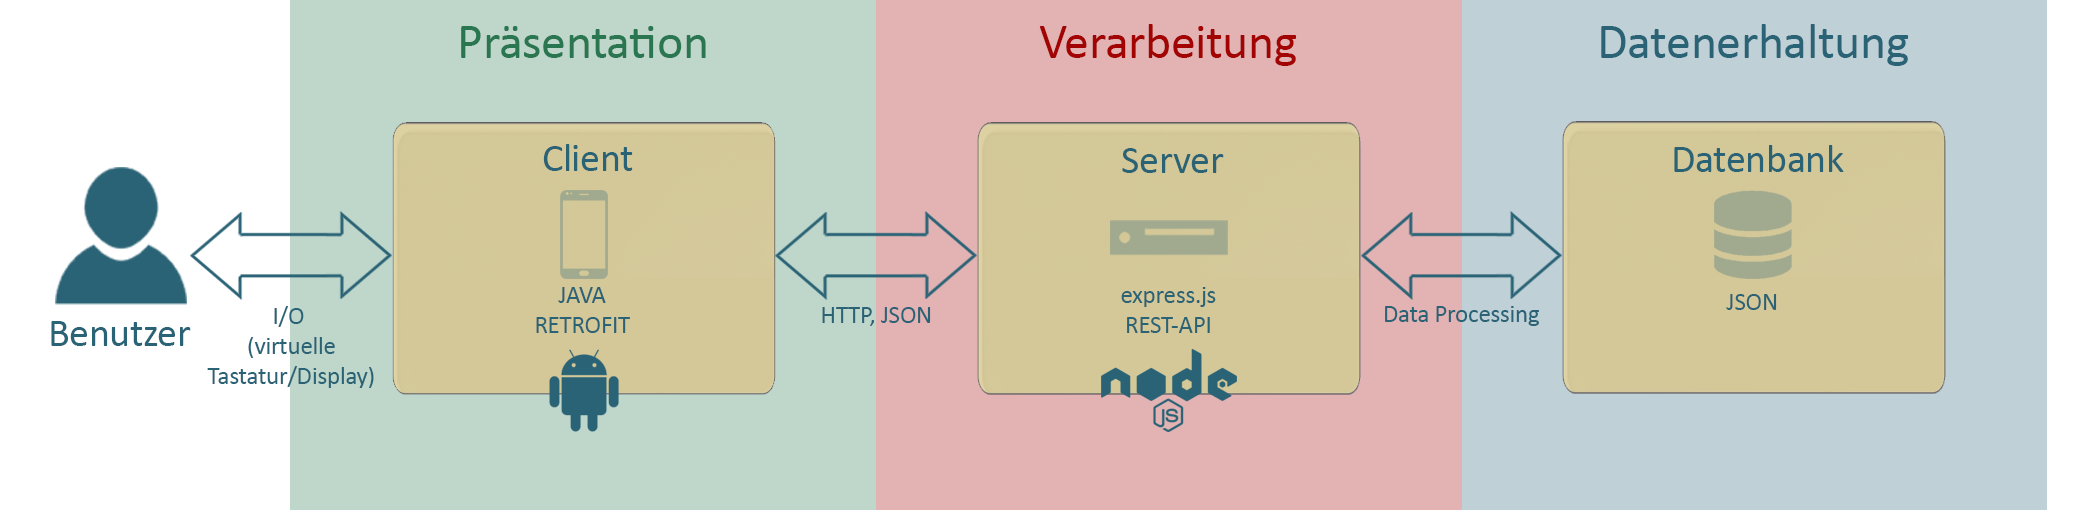
\includegraphics[width=1.0\textwidth]{images/funktionsweise.png}}
	 \captionsetup{justification=centering}
	 \caption{Funktionsweise}
	 \label{img:funktionsweise}
	 \end{figure}
	 
	 \subsection{Installationsdokumentation}
	 Um das System erfolgreich installieren zu können, muss zunächst muss das GitHub-Repository geklont werden. Das Repository kann in der Shell mit folgenden Befehl geklont werden:\\	 
	 \textit{\$ git clone https://github.com/sami1905/BAWS1920Hassini}\\
	 Nun folgt die Beschreibung, mit der Server und Client installiert werden können.
	 \subsubsection{Server}
	 1. Starte die Shell und öffne den Pfad:\\
	 \textit{/Implementation/DiaLog/Server}\\
	 2. Starte den Server mit dem Befehl:\\
	 \textit{\$ node app.js}\\
	 3. Sobald die Meldung \textit{\glqq Server läuft auf Port 3000.\grqq{}} in der Shell erscheint, ist der Server erfolgreich installiert und gestartet.
	  \subsubsection{Client}
	  1. Android Studio starten und den Odner \textit{Client} aus dem Repository öffnen.\\
	  2. Ein Virtual Device einrichten.\\
	  3. Emulator starten.\\
	  4. Um das System verwenden zu können, mit der E-Mail-Adresse \textit{\glqq m.mustermann@th-koeln.de\grqq{}} und dem Passwort \textit{\glqq 12345678\grqq{}} anmelden.
	
